% Toolbar icon: cad — a faceted triangle patch turned into a smooth analytic
% solid (a shaded cylinder: the primitive fitCad fits), with an arrow between.
% Same coarse → arrow → result language as remesh.tex.
\documentclass[tikz,border=2mm]{standalone}
\usetikzlibrary{arrows.meta,calc,shapes.geometric}
\begin{document}
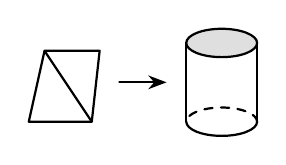
\begin{tikzpicture}[line width=1.3pt, line cap=round, line join=round, >=Stealth, x=1mm,y=1mm]
  % --- faceted patch (two triangles) ---
  \coordinate (A) at (-16,-5);
  \coordinate (B) at (-8,-5);
  \coordinate (C) at (-14,4);
  \coordinate (D) at (-7,4);
  \draw[thick] (A) -- (B) -- (D) -- (C) -- cycle;
  \draw[thick] (B) -- (C);
  % --- arrow ---
  \draw[thick,->] (-4.5,0) -- (1.5,0);
  % --- smooth cylinder: shaded top face, body, solid front / dashed back base ---
  \draw[thick,fill=gray!25] (8.5,5) ellipse (4.5 and 1.8);
  \draw[thick] (4,5) -- (4,-5);
  \draw[thick] (13,5) -- (13,-5);
  \draw[thick] (4,-5) arc (180:360:4.5 and 1.8);
  \draw[thick,dashed] (13,-5) arc (0:180:4.5 and 1.8);
\end{tikzpicture}
\end{document}
